%%%%%%%%%%%%%%
%%  Template for latex documents
%%  Author: Marco A. Aquino-Lopez
%%  Nota: to get a word document use pandoc
%%  pandoc -f latex Articulo.tex -o Articulo.docx --bibliography=bibliography.bib
%%%%%%%%%%%%%%%%%
%\documentclass [twocolumn,10pt] {article}
\documentclass [10pt] {article}

\usepackage [utf8] {inputenc}
\usepackage[english]{babel}

\usepackage {graphicx}
%\usepackage {amsfonts,unicode-math}
\usepackage {amsthm}
\usepackage {amsmath}
\usepackage {natbib}

\usepackage{hyperref}
\usepackage[in]{fullpage} %To have more in the page
%.____         ___________    ____  ___ 
%|    |   _____\__    _______ \   \/  / 
%|    |   \__  \ |    |_/ __ \ \     /  
%|    |___ / __ \|    |\  ___/ /     \  
%|_______ (____  |____| \___  /___/\  \ 
%        \/    \/           \/      \_/ 

\graphicspath{{Figures/}} %Setting the graphicspath

%Extra packages2
\usepackage{placeins}

%%%%%%

\date{ }
\usepackage{color}

%%%% To mark notes or added text by Author1 (a1)
%%%% This allows to add notes
%\newcommand{\a1}{\color{red} }  %% begin
%\newcommand{\1a}{ \color{black}} %% end
%\newcommand{\cuta1}[1]{\ac [cut] \ca} %% to mark cut text
%\newcommand{\notea1}[1]{\textcolor{red}{(note)}\footnote{\ac #1 \ca}}  %% To add a note or comment

% %%%% To mark notes or added text by Andres (ac)
 \newcommand{\ac}{\color{red} }  %% begin
 \newcommand{\ca}{\color{black}} %% end
 \newcommand{\cutac}[1]{\ac [cut] \ca} %% to mark cut text
 \newcommand{\noteac}[1]{\textcolor{red}{(note)}\footnote{\ac #1 \ca}}  %% To add a note or comment

% %%%% To mark notes or added text by Marco (ma)
% \newcommand{\ma}{\color{blue} }  %% begin
% \newcommand{\am}{\color{black}} %% end
% \newcommand{\cutma}[1]{\ac [cut] \ca} %% to mark cut text
% \newcommand{\noteam}[1]{\textcolor{red}{(note)}\footnote{\ac #1 \ca}}  %% To add a note or comment


% NOTE: To produce blinded version, replace "0" with "1" below.
\newcommand{\blind}{1}
\newcommand{\papertitle}{
	Decoding Peatland Dynamics: A Bayesian Model for Inferring System Shifts and Carbon Decomposition
}

\begin{document}
	\def\spacingset#1{\renewcommand{\baselinestretch}%
		{#1}\small\normalsize} \spacingset{1}
	%%%%%%%%%%%%%%%%%%%%%%%%%%%%%%%%%%%%%%%%%%%%%%%%%%%%%%%%%%%%%%%%%%%%%%%%%%%%%%
	\if1\blind
	{
		\title{\textbf{\papertitle}}

		\author{Marco A Aquino-L\'opez\thanks{
				Department of Geography, University of Cambridge, 
				Cambridge, United Kingdom
				email: \texttt{aquino@cimat.mx} } \thanks{Corresponding author.}
					\and
			Jingjing Sun\thanks{
				Northeast Normal University
				China. 
				email: \texttt{sunjj878@nenu.edu.cn}}
					\and
			Angela \thanks{
				Exeter University
				United Kingdom.
				email: \texttt{}  }
			}
		\maketitle
	} \fi

	\if0\blind
	{
		\bigskip
		\bigskip
		\bigskip
		\begin{center}
			{\LARGE\bf \papertitle}
		\end{center}
		\medskip
	} \fi
\bigskip

\begin{abstract}
This paper introduces a novel Bayesian model designed to provide a sophisticated understanding of carbon dynamics within peatland ecosystems. Our model takes inspiration from the classic Clymo model, while addressing some limitations of the traditional approach. Specifically, the new model allows for the variable influxes of carbon, even in the deepest sediment layers, offering a more realistic and nuanced portrayal of carbon behaviour in peatlands.

We introduce a novel aspect: a weighted function that is instrumental in defining a boundary between two distinct systems within the peatland, but also allows for a smooth transition from one system to another. This feature is particularly relevant in scenarios where a shift in the water table leads to a significant difference in decomposition rates above and below the water line.

	Our model embraces the complexity of peatlands and underscores the importance of Bayesian statistics for making accurate inferences about system shifts and carbon decomposition in these vital ecosystems. The paper further elaborates on the theoretical underpinnings of the model, its application, and the implications of our findings for peatland management and carbon cycle science. With this work, we aim to provide a robust tool for advancing research on peatland dynamics and their role in the global carbon cycle. 

\end{abstract}
	\noindent%
	{\it Keywords:} Clymo model, carbon accumulation, Bayesian statistics	\vfill
	\newpage
	\spacingset{1.45} % DON'T change the spacing!

\section{Introduction}
Peatlands play a crucial role in the global carbon cycle, acting as significant carbon sinks that help mitigate the impacts of climate change. Understanding the intricate dynamics of carbon influx and decomposition in these ecosystems is paramount for developing effective strategies for their management and conservation. However, carbon dynamics in peatlands can be complex, affected by myriad variables and processes occurring at different layers of the ecosystem.

Traditional models, such as the Clymo model, have provided valuable insights into these dynamics, but they often fall short in capturing the variable nature of carbon influxes, particularly in the deepest parts of peatland sediments. Furthermore, these models typically delineate sharp boundaries between different systems within peatlands, neglecting the gradual transitions that often occur in reality.

In response to these limitations, this paper introduces a novel Bayesian model for inferring system shifts and carbon decomposition in peatlands. This model is built upon the foundations of the Clymo model but extends its capabilities by incorporating a weighted function to allow for a smooth transition between different systems. This is especially relevant when considering phenomena like changes in the water table, which can drastically alter the decomposition rates above and below the water line.

The remainder of this paper is organized into four chapters, each focusing on a key aspect of our research: Chapter 2 delves into the specifics of the data utilized for this study and discusses the problems and limitations associated with conventional peatland carbon models, and the need for an improved, more nuanced approach. Chapter 3 details the development and structure of the Bayesian model. It presents the mathematical and theoretical foundations of the model, and outlines the innovative use of a weighted function to infer system transitions in peatland ecosystems. Chapter 4 provides a comparative analysis of our model's performance relative to traditional models. We demonstrate the enhanced capabilities of our model, particularly in modelling variable carbon influxes and smooth system transitions. Chapter 5 summarizes the findings of our study and discusses their implications for peatland management and carbon cycle research. 


\section{Carbon estimation: Data and Problems}

\section{Model Construction}


\subsection{weighted function}

\begin{figure}
	\begin{centering}
		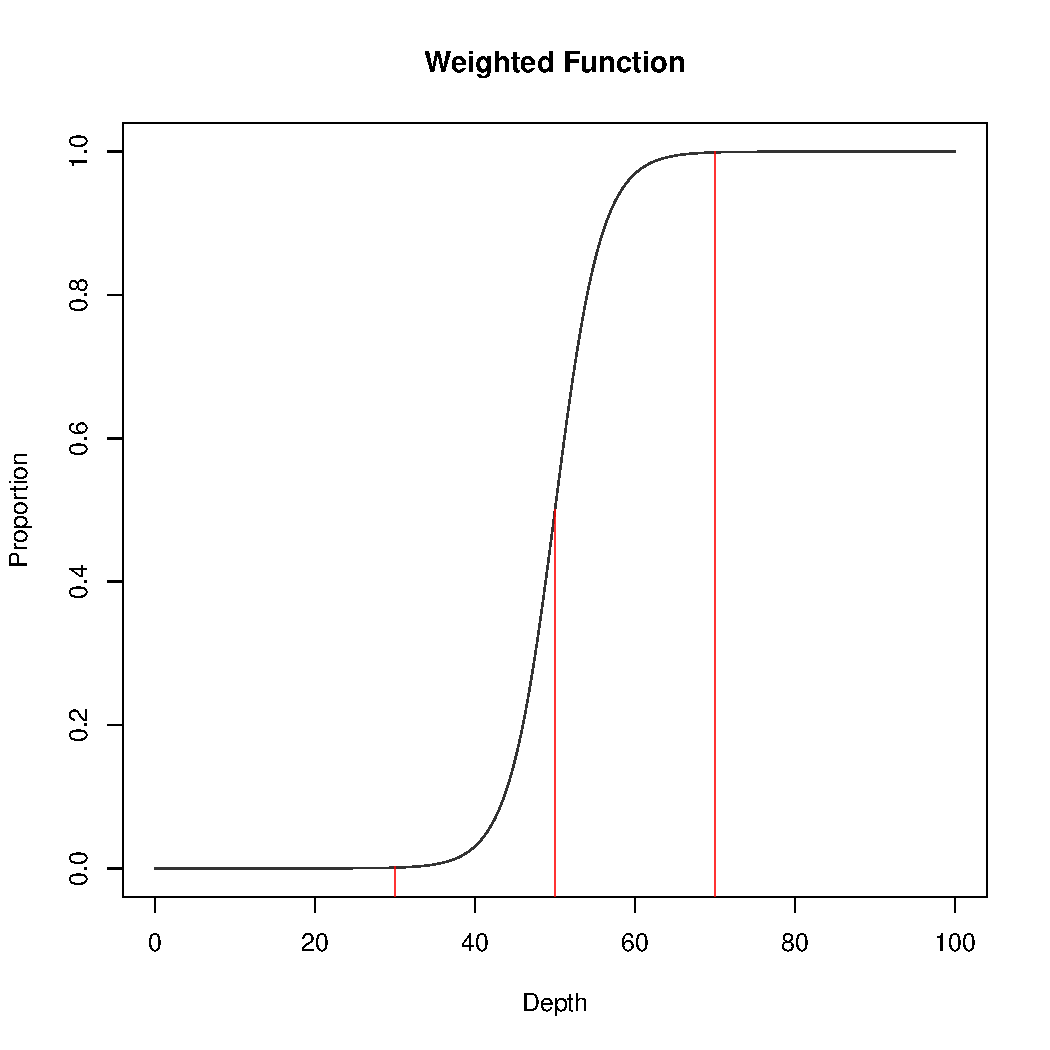
\includegraphics{weighted_fun.pdf}
		\caption{representation of the weighted function with a boundary at depth 50 and 20 cm of delay.}
		\label{}
	\end{centering}
\end{figure}





\section{Comparison}







\section{Conclusion and Discussion}












\bibliographystyle{apalike}
\bibliography{bibliography.bib}
\newpage


\end{document}

